\documentclass[10pt,conference]{IEEEtran}
\IEEEoverridecommandlockouts % show footnote comments
% =============================================================
%         setting for IEEE format paper (normal mode)
%
%   Author      : Bei Yu
%   Last Update : 02/2021
% =============================================================

\usepackage{blkarray}                                      % to support matrix
%\usepackage[noend]{algpseudocode}
\usepackage{algpseudocode}                                 % new algorithm package
\usepackage{algorithm}
\usepackage{graphicx}                                      % include pdf figures
\usepackage{amsmath}
\usepackage{amssymb}
\usepackage{amsfonts}
\usepackage{amsthm}
\usepackage[mathcal]{eucal}
\usepackage{booktabs}
\usepackage{enumerate}
\usepackage{multirow}
\usepackage[subrefformat=parens,farskip=0pt,justification=centering]{subfig}
\captionsetup[subfigure]{labelformat=simple}               % avoid "double brackets" in sub-figure caption
\renewcommand\thesubfigure{(\alph{subfigure})}             % "Fig.~1b"-->"Fig.1(b)"
\usepackage{color}
\usepackage{cite}                                          % more citations in one bracket
\usepackage{comment}                                       % use comment
\usepackage{soul}                                          % use highlight command \hl{}
\soulregister\cite7
\soulregister\ref7
\soulregister\pageref7
\usepackage{etoolbox}                                      % commands \newtoggle, \toggletrue, \iftoggle
\usepackage{url}
\usepackage{nth}                                           % nth command
\usepackage{bm}                                            % bm command
\usepackage{courier}
\usepackage{balance}
\usepackage{threeparttable}
\usepackage[bookmarks=false]{hyperref}
\hypersetup{
    colorlinks = true,
    citecolor  = blue,
    linkcolor  = blue,
    urlcolor   = blue,
}
\usepackage{tikz}
\usetikzlibrary{positioning,calc,fit,decorations.pathmorphing}
\usepackage{filecontents}                                  % support to pgfplots
\usepackage{pgfplots}
\usepackage{pgfplotstable}
\usepackage{scalefnt}
\pgfplotsset{compat=newest}
\usepackage{caption}
\usepackage{cleveref}
\Crefformat{figure}{Fig.~#2#1#3}                           % "Fig.", instead of "Figure"
\Crefname{subfigure}{Fig.}{Figs.}
\Crefname{figure}{Fig.}{Figs.}
\Crefformat{table}{TABLE~#2#1#3}                           % "TABLE", instead of "Table"
\captionsetup[table]{skip=4pt}
\captionsetup{labelsep=space}

% ==== local color definitions
\definecolor{CUHKorange}{RGB}{244,106,18} %F47012
\definecolor{CUHKblue}{RGB}{0,111,190}    %006FBE
\definecolor{CUHKgreen}{RGB}{0,127,128}   %007F80
\definecolor{CUHKred}{RGB}{228,46,36}     %E42E24
\definecolor{CUHKyellow}{RGB}{198,148,34} %C69422
\definecolor{CUHKdark}{RGB}{114,44,114}   %722C72
\definecolor{CUHKmiddle}{RGB}{144,44,144} %902C90
\definecolor{CUHKlight}{RGB}{167,44,167} 

% ==== Local new commands
\newcommand{\calH}{\mathcal{H}}
\newcommand{\calL}{\mathcal{L}}
\newcommand{\calN}{\mathcal{N}}
\newcommand{\calO}{\mathcal{O}}
\newcommand{\calP}{\mathcal{P}}
\newcommand{\calQ}{\mathcal{Q}}
\newcommand{\calV}{\mathcal{V}}
\newcommand{\calKL}{\mathcal{KL}}
\newcommand{\norm}[1]{\left\lVert#1\right\rVert}
\renewcommand{\vec}[1]{\boldsymbol{#1}}    % re-define vec command
\DeclareMathOperator*{\argmin}{argmin}


% =============================================================
%              page size setting (in normal mode)
% =============================================================
\setlength{\columnsep}{18pt}                               % set space between columns
% =============================================================
%                   Theorem Definitions
% =============================================================
\newtheorem{myproblem}{\textbf{Problem}}
\newtheorem{mydefinition}{\textbf{Definition}}
\newtheorem{mytheorem}{\textbf{Theorem}}
\newtheorem{mycorollary}{\textbf{Corollary}}
\newtheorem{mylemma}{\textbf{Lemma}}
\newtheorem{myclaim}{\textbf{Claim}}
\newtheorem{myapplication}{\textbf{Application}}
\newtheorem{myexample}{\textbf{Example}}
\newtheorem{myconjecture}{\textbf{Conjecture}}
\newtheorem{myassumption}{Assumption}
\newtheorem{myprop}{Property}

\algrenewcommand\textproc{\texttt}
\newcommand{\tabincell}[2]{
    \begin{tabular}{@{}#1@{}}#2\end{tabular}
}

% long line in algorithm
% e.g.: \Statex[4] ...;
\makeatletter
\let\OldStatex\Statex
\renewcommand{\Statex}[1][3]{%
  \setlength\@tempdima{\algorithmicindent}%
  \OldStatex\hskip\dimexpr#1\@tempdima\relax
}
\makeatother


% =============================================================
%          Definitions to support latexdiff
% =============================================================
%DIF PREAMBLE EXTENSION ADDED BY LATEXDIFF
%DIF UNDERLINE PREAMBLE %DIF PREAMBLE
\RequirePackage[normalem]{ulem} %DIF PREAMBLE
\RequirePackage{color}\definecolor{RED}{rgb}{1,0,0}\definecolor{BLUE}{rgb}{0,0,1} %DIF PREAMBLE
\providecommand{\DIFadd}[1]{{\protect\color{blue}{#1}}}                           %DIF PREAMBLE
\providecommand{\DIFdel}[1]{{\protect\color{red}\sout{#1}}}                       %DIF PREAMBLE
%DIF SAFE PREAMBLE %DIF PREAMBLE
\providecommand{\DIFaddbegin}{}                                                   %DIF PREAMBLE
\providecommand{\DIFaddend}{}                                                     %DIF PREAMBLE
\providecommand{\DIFdelbegin}{}                                                   %DIF PREAMBLE
\providecommand{\DIFdelend}{}                                                     %DIF PREAMBLE
%DIF FLOATSAFE PREAMBLE %DIF PREAMBLE
\providecommand{\DIFaddFL}[1]{\DIFadd{#1}}                                        %DIF PREAMBLE
\providecommand{\DIFdelFL}[1]{\DIFdel{#1}}                                        %DIF PREAMBLE
\providecommand{\DIFaddbeginFL}{}                                                 %DIF PREAMBLE
\providecommand{\DIFaddendFL}{}                                                   %DIF PREAMBLE
\providecommand{\DIFdelbeginFL}{}                                                 %DIF PREAMBLE
\providecommand{\DIFdelendFL}{}                                                   %DIF PREAMBLE
%DIF END PREAMBLE EXTENSION ADDED BY LATEXDIFF


% =============================================================
%          Local revision functions 
% =============================================================
\newcommand{\todo}[1]{\textcolor{red}{[TODO: #1]}}
\newcommand{\revise}[1]{\DIFadd{#1}}

% ==== Logs:
%
%  01/2020: todo & revise functions
%  02/2019: vec commend
%  10/2018: captionsetup: remove ":" in caption; eucal package
%  09/2016: captionsetup, columnsep
%  07/2016: support to pgfplots
%  07/2016: threeparttable
%  04/2016: definitions supporting latexdiff
%  04/2016: remove bookmarks in hyperref
%  02/2016: tabincell
%  02/2016: hyperref
%  12/2015: copy from "ieee_conference"
%


\usepackage{graphics}
\graphicspath{{./figs/}}

\usepgfplotslibrary{groupplots}
\usetikzlibrary{patterns}

% pseudocode 
\usepackage{algorithm}
\usepackage{algpseudocode}
\usepackage{amsmath}
\usepackage{setspace}
\renewcommand{\algorithmicrequire}{\textbf{Input:}}  % Use Input in the format of Algorithm
\renewcommand{\algorithmicensure}{\textbf{Output:}} % Use Output in the format of Algorithm


% ==== Local defined colors
\definecolor{mypink}{RGB}{255,171,164}     %FFABA4
\definecolor{mygray}{RGB}{240,240,240}     %F0F0F0\subsubsection{} \\

\definecolor{lightblue}{RGB}{221,239,250}  %DDEFFA
\definecolor{myred}{RGB}{228,46,36}        %E42E24
\definecolor{mygreen}{RGB}{142,202,206}    %8ECACE
\definecolor{myyellow}{RGB}{255,253,181}   %FFFDB5
\definecolor{myblue}{RGB}{71,162,241}      %47A2F1

\definecolor{myorange}{RGB}{244,106,18}
\definecolor{mylight}{RGB}{191,191,255}

\begin{document}

\title{
    % AutoGTCO: Graph and Tensor Co-Optimize for Image Recognition with Transformers on GPU
    AutoGTCO: Design and Generation of Efficient Tensor Programs for Image Recognition with Transformers on GPU
}

\iffalse
\author{
    Yang Bai$^1$, \quad
    Bei Yu$^1$ \\
    $^1$The Chinese University of Hong Kong \qquad
    %$^2$Hisilicon Technologies Co.\\
    {\tt\small \{ybai,byu\}@cse.cuhk.edu.hk}
}
\fi


\maketitle


\begin{abstract}  

Performance optimization is the art of continuous seeking an effective mapping between algorithm and hardware. Existing deep learning compilers or frameworks optimize
the computation graph by adapting transformations manually designed by high-performance computing engineer efforts. This method misses some possible graph-level optimizations,
and it is difficult to generalize to emerging deep learning models or new operators. 
In this work, we propose AutoGTCO, a tensor program generation system for image recognization with transformer architectures on GPU. Compared with existing fusion strategies,
AutoGTCO explores optimization of operator fusion in transformer model through a novel dynamic programming algorithm. In order to construct an effective search space of the sampled programs, new sketch generation rules and a search policy are proposed for the batch matrix 
multiplication and softmax operators in each subgraph, which are capable of fusing them into large computation units, then mapping and transforming them into 
efficient CUDA kernels. Overall, our evaluation on three real-world image recognization tasks shows that AutoGTCO improves the end-to-end execution performance of transformer model relative to 
the state-of-the-art deep learning library TensorRT on NVIDIA GPU by up to 1.27x.
  

\end{abstract}



\section{Introduction}

Recent years have witnessed a surge of industry scale applications of machine learning models, ranging from autonomous driving, augmented 
reality, language translation, to billion scale search and recommendation systems. Such workloads can be expressed as a directed acyclic 
computational graph (DAG) by high level Python APIs, in which nodes verbalize the operators and edges represent the relationship between
adjacent operators. These computational graphs are mapped to hardware accelerators (such as GPUs) through existing deep learning frameworks
(such as TensorFlow, PyTorch, Caffe) by vendor-provided kernel libraries (such as cuDNN, MKL-DNN, ARM-Compute Library) to achieve high
performance. These kernel libraires need significant engineering effort to manually tune for different operators on a diversity
of hardware platforms. \\

Currently, dense tensor computations (such as matrix multiplication, convolution) are ubiquitous in deep learing workloads. Thus researchers
and engineers either focus on optimizing performance of such compute intensive primitives, or turning to search-based compilation by decoupling the kernel definitation and computation scheduling for automated generation of tensor programs. This approach performs well for workloads which 
are dominated by FLOPs. Take NVIDIA TensorRT as example, it uses two steps to optimize the computational graph which is built with deep learning 
frameworks. In the first step, some operators are fused vertically by the specific rules designed by the high-performance computing engineers. In the second step, the fused operators in the same level are fused horizontally. Existingdeep learning systems such as TensorFlow, PyTorch, and
TVM optimize an input computation graph by performing greedy rule-based substitutions on the graph. Each substitution
replaces a subgraph matching a specific pattern with a new subgraph that computes the same result. For example, operator fusion combines several operators into one, which can eliminate intermediate results and increases the granularity of the operators, thereby reducing system overheads such as memory accesses and kernel launches. However, the challenge is how to transform high level computation graphs into efficient kernels in
order to maximize the execution efficiency on deep learning accelerators. \\


To address this challenge, we introduce xxx, an operator fusion strategy that accelerates Transformer model inference by exploring the opportunities of combination automatically between adjacent operators. In our experiments, we find that different operator fusion strategy share
common sub-schedules. Therefore, we model this process as a multi-stage decision problem and adopt dynamic programming technique to search the 
optimal operator fusion strategy with a low computation cost. We evaluate our method on xxx a

In summary, this paper makes the following contributions:
\begin{itemize}
  \item We introduce a novel dynamic programming algorithm to solve the operator fusion problem for transformer models. This technique can automatically generate the optimal combination for operators in the subgraph-level, which explores a large combination space than the rule-based method defined by high-performance computing engineers in the deep learning compiler.
  \item Based on Ansor, we propose new sketch generation rules and a search policy for the batch matrix multiplication and softmax operators in subgraphs. This mechanism constructs an effective search space of tensor programs for the kernel generation. In order to get a high-performance and end-to-end compilation flow, a learned cost model is used to fine-tune the performance of each kernel.
  \item We apply our method to currently popular image recognition tasks with transformer models (such as DETR, SETR, ViT). Our method can automatically generate corresponding CUDA code on GPU under different inference configurations.
  The optimized CUDA code consistently outperform the state-of-the-art deep learning library TensorRT with xxx measured speedup in the 
  inference stage.
\end{itemize}

\label{sec:intro}



\section{Background and Motivation}
\label{sec:bkg}

Here, we provide a brief overview of our terminology, transformers, and xxx. We assume that the readers are generally familiar with how to train and inference
deep neural networks on NVIDIA GPUs.


% \subsection{Object Detection and xxx}

% The target of object detection is to predict a set of bounding boxes and labels for each substance in an image. Modern object detectors solve this problem 
% in a redundant way, by pre-defining a large set of proposals, anchors to address regression problem for the location of coordinates and classification problem 
% for the category labels. The performance of this model is significantly influenced by postprocessing steps to suffer from strong similarity predictions, by the
% design of deploymenting anchors and by the strategy that assign predicted boxes to anchors.

% \textbf{faster rcnn based approach}

% \textbf{detr based approach}

\begin{figure*}[htbp]
    \centering
    \label{fig:fig6}
    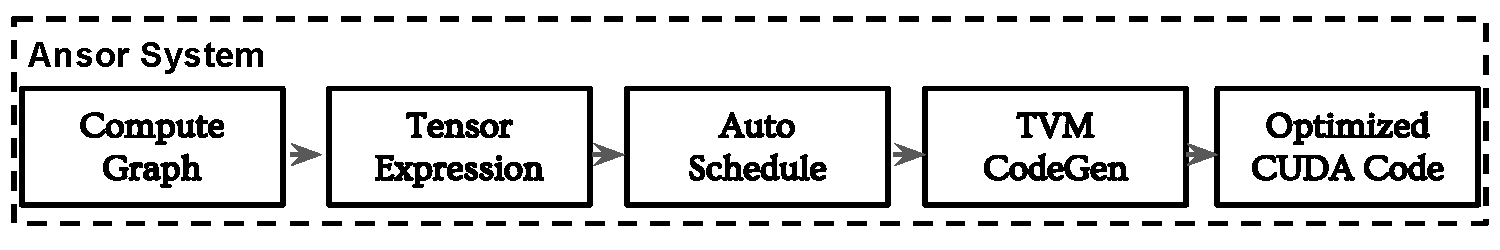
\includegraphics[height=3cm, width=15cm]{figs/fig6}
    \caption{The System Overview of Ansor. First, the input of Ansor is computation graph and it is converted into tensor expression language. Second, Auto-Schedule module
    can search the optimial schedule automatically for the tensor expression language. Finally, TVM code generation can generate optimized CUDA code on GPU backend 
    for the computation graph.}
\end{figure*}
\subsection{Image Recognition}
{\color{red} Image Classification, Object Detection, Semantic Segmentation}

Image recognition has been significantly boosted with the development of deep neural networks. There are three particularly important 
tasks in image recognition: (1) Image classification, (2) object detection, and (3) semantic segmentation. Image classification can classify what is contained in an image. Object detection is a combination of image location and classification. Image localization specifies the location of single object in an image whereas object detection specifies the location of multiple objects with their labels in the image. Image segmentation creates a pixel wise mask of each object in the image. Note that all popular approaches are still based on convolutional neural network where the feature encoding and extraction part are based on classical ConvNets like ResNet and VGG.

\subsection{Transfomers}

The transformer model, originally developed for a new attention-based building block for machine translation, or transforming an input sequence into an output 
sequence. Transformers build on a long sequence within natural language processing, most relevantly starting with word embeddings, neural machine translation, and 
sequence-to-sequence learning. The key element in transformer architecture is attention part, which is composed of neural networks layers that aggregate 
information from the entire input sequence and make model to learn to focus on particular parts of a sequence. One of the important advantages of attention-based model is their global computations and perfect memory scheduling, which leads them more eligible than 
RNNs on long sequences. Transformer models make two mian contributions. The first one is that it popularizes attention mechanisms to a particular module named 
\textit{multi-head attention}. The second one is that it does not rely on recurrent or convolutional algorithms, but completely relies on attention mechanisms. 
Most importantly, many similar architecture of subgraphs in transformer model can greatly reduce the tuning time for the kernel with the same configuration and run
parallelly, which we discuss below.

\textbf{Encoder:} The encoder module is composed of a stack of identical layers. There are two sub-layers in each layer. The first sub-layer is a multi-head 
attention mechanism, and the second sub-layer is a simple, positionwise fully dense layer. A residual connection layer is used between each of the two sub-layer
with a layer normalization. That is to say, the output of each sub-layer is actually the sum of the input and the attention of input under the layer normalization.
And the output of dimension is defined as $d_{model}$

\textbf{Decoder:} The structure of the encoder and decoder is very similar. The decoder is also composed of a stack identical layers. In addition to the two subl-layers
mentioned in the encoder module, a third sub-layer is inserted into the decoder module. The function of the third sub-layer is to perform multi-head attention over the 
output of the encoder part. At the same time, some modifications about masking mechanisms in the self-attention sub-layer is to prevent positions from attending to subsequent positions.
It combines with the fact that the output of embedding layers are offset by one position, and it is ensured that the perdiction of the \textit{i-}th position only 
depends on the known outputs less than the \textit{i-}th positions.

\textbf{Multi-head Attention:} Multi-head Attention generalizes attention mechanisms, and employs \textit{h} attention heads parallelly to get 
different learnt projections of a given sequence. Each attention head is an instance of \textit{scaled dot-product attention}, and takes queries (q),
keys (k), values (v) as its input. The function of attention is to find values corresponding to the keys closest to the input queries. The function of 
heads are also augmented with linear layers that project their inputs into a lower-dimensional space. The three inputs are first multiplied by weight
tensors \textit{wq}, \textit{wk}, \textit{wv}, respectively, as a learned input projection. The query and key tensors are subsequently multiplied together
and scaled, followed by applying the softmax operation in order to weight and select the most relevant results. This is then multiplied with \textit{vv} to 
produce the per-head output. The outputs of all the heads are finally concatenated and linearly projected back to the input dimensional size.
Multi-head attention may also have a masking step, which is used during the training stage to prevent the model from seeing the future information
and using message from a later part of a sequence. 



\textbf{Transformer Architecture:}
 A transformer architecture is composed of both encoder and decoder modules. It is worth noting that transformer-based model does not necessarily have 
decoder module. For instance, the widely used BERT model does not have this structure.


\subsection{Deep Learning Compiler}
\textbf{Ansor:} Ansor is equipped with a hierarhcical search space that decouples high-level structures and low-level details. 
Ansor constructs the search space for a computational graph automatically, 
eliminating the need to manually develop high-performance computing templates by the experienced engineers. 
It then uses auto-tuner to sample complete programs from the search space and implements fine-tuning on complete programs under the XGBoost cost model. 
Figure \ref{fig:fig6} shows the overall architecture of Ansor.




\subsection{Hierarchy of 2080Ti GPUs}
Compute Unified Device Architecture (CUDA) is a parallel computing platform and programmming model for GPUs, which exposes high-performance computing programmers
to the concepts of memory hierarchy and threads hierarchy. Accelerating deep learning performance on complex memory hierarchy needs to make good use of memory
units and compute units. 
\begin{figure}[htbp]
    \centering
    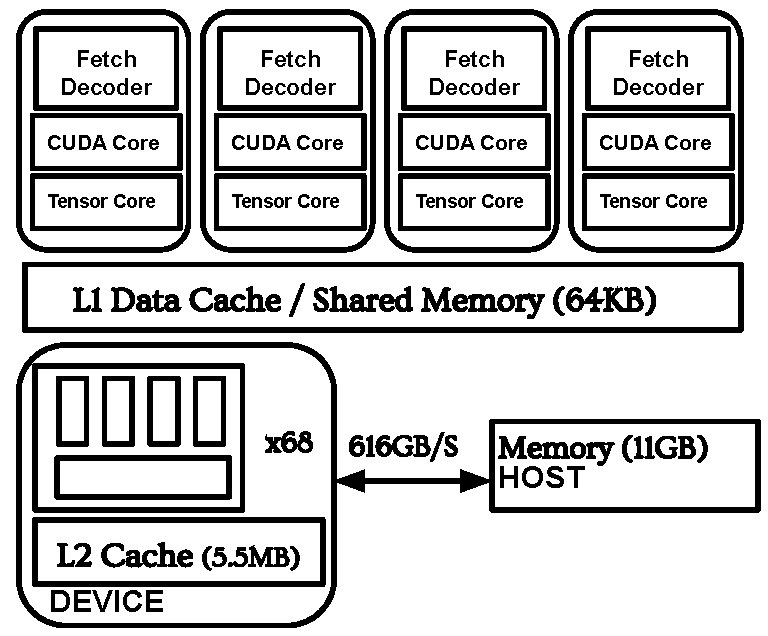
\includegraphics[height=5cm, width=6cm]{figs/fig5}
    \caption{A streaming multiprocessor and the architecture in GeForce RTX 2080 Ti GPU}
    \label{fig5}
\end{figure}
As shown in Figure \ref{fig5}, there are many programmable memories at different levels of GPU devices. GPU memory units are different from access pattern to management.
NVIDIA 2080Ti GPU contains 68 Stream Multiprocessors(SMs) which can run parallelly on the board. Each SM has its shared memory, which can be accessed by threads
in the same block. A SM is partitioned into multiple blocks and each block can only access its private shared memory. Registers and local memory can only be visited
by a single thread. If the size of the required memory is larger than the size each thread allocated, local memory in each block will be used. Generally, data copying
from host memory to device memory will be executed before the computation kernel is launched. \\
On-chip memory is fast and adjacent to chips whereas off-chip memory is slow and far away from chips. Different types of memory have different access patterns.
Registers and local memory in the same block are both private to each thread. Registers are on-chip with low latency. Shared memory is organized by a full-sized 
replica of banks. Simultaneous data accessing by different threads to the same bank will lead to a shared memory bank conflict problem, and it gives rise to
higher latency. 
% \textbf{\subsection{Challenges with End-to-End Optimization}}


\section{Problem Definition}

This section defines the graph fusion schedule and formulates the problem.

\textbf{Computation Graph.}
Computation graphs are a common way to represent prgrams in deep learning frameworks.
A transformer model is defined by a computation graph $G=(V, E)$, where $V$ is the set of vertices. Each vertex can represent an operator such as gemm and convolution
opertation in the computation graph. And $E$ is the set of edges which can describe the relationship between a pair of vertices. Each edge $(u, v)$ is a tensor that can 
store the output of operator $u$ and the input of operator $v$. 
Figure \ref{fig:fig1} shows the computation graph of the encoder in transformer model. \\

\begin{figure}[htbp]
    \centering
    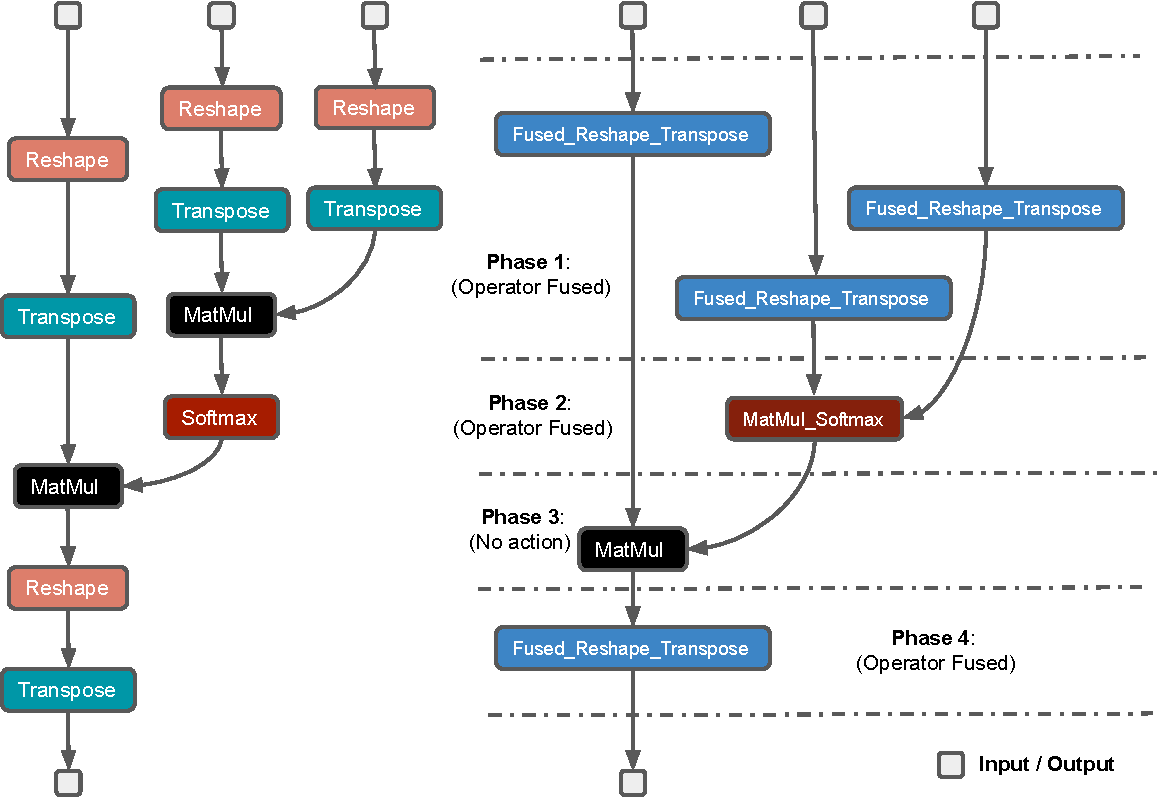
\includegraphics[width=.98\linewidth]{fig1}
    \caption{xxx}
    \label{fig:fig1}
\end{figure}


\textbf{Operator Pattern.}
Operator fusion combines multiple operators which are in adjacent positions into a single kernel rather than storing the intermediate results in the 
global memory. This optimization can greatly improve speed-up, particularly in throughput oriented architectures such as GPUs. In order to combine operators
efficiently, we should define the pattern of each operator in the computation graph. Specificaly, we set the transfomer model as our optimization goal. In TVM, 
it recognize four categories of graph opertators: (1) \textit{injective} (one-to-one map), (2) \textit{reduction}, (3) \textit{complex-out-fusable} (can fuse
element-wise map to output), and (4) \textit{opaque} (can not be fused by any operator). And it provides generic rules to fuse these operators. From
the background section, we know that transpose of matrix, batch matrix multiplication, layer normalization, softmax, and dense layer occur frequently in the 
transformer computation graph. In the meantime, the default configuration of the operators in TVM are as follows. Softmax is tagged as opaque pattern.
Batch matrix multiplication and dense are tagged as complex-out-fusable pattern. Layer normalization can be decomposed to be a set of add/subtract/multiple operators
which are all tagged as element-wise pattern. The fusion strategy is discussed below. \\


% injective, 
% reduction, 
% complex-out, 
% opaque
% # Elementwise operator
% ELEMWISE = 0
% # Broadcast operator
% BROADCAST = 1
% # Injective mapping
% INJECTIVE = 2
% # Communication
% COMM_REDUCE = 3
% # Complex op, can still fuse ewise into it
% OUT_ELEMWISE_FUSABLE = 4
% # Represents tuple node
% TUPLE = 7
% # Not fusable opaque op
% OPAQUE = 8


\textbf{Fusion Strategy and Schedule.} 
We define a schedule $S$ of a computation graph $G$. The scheduling can be defined as:
\begin{equation}
    S = \left\{(V_1, F_1), (V_2, F_2), ..., (V_k, F_k)\right\},
\end{equation}
where $V_k$ represents a group of computation operators in the \textit{i}-th phase and $F_k$ is a pair to descirbe the fusion relationship between node $v_i$
and $v_j$. For instance, the schedule for Figure xxx can be sketched by xxx.
Computation graph can be executed under the schedule $S$ from the first phase $(V_1, F_1)$ to the last phase $(V_k, F_k)$ consecutively.\\

% some common schedules for tensor program generation:split, reorder, fuse, compute_at, tile, parallel, vectorize, unroll, bind, compute_inline


\textbf{Problem Formulation.}
In order to reduce the runtime of the whole compuation graph on GPU, we set $Cost$ as a cost function on a computation graph $G$ and 
fusion schedule $S$. Our goal is to find a schedule $S^*$ to minimize the cost function for a computation graph $G$.

\begin{equation}
    {S^*} = \mathop{argmin}\limits_{S} \ Cost(G, S)
\end{equation}
The goal of the optimization is to make computation graph have low latency on the NVIDIA GPU. Therefore, we use the latency of executing executing computation 
graph $G$ according to schedule $S$ as the cost function. \\




\label{sec:form}

\section{Our Method}

\subsection{Overview}

{\color{red} Using DETR model as our example to verify the acceleration of transformer, }

The overall DETR architecture is surprisingly simple and described in Figure xxx. It contains three main components, which we represent below:
a CNN backbone to extract a compact feature map, an encoder-decoder transformer model, and a simple feed neural network (FFN) which is composed
of two-layers of $1 \times 1$ convolutions with ReLU activation functions. In this work, we take DETR as our example to accelerate the inference
time on NVIDIA GeForce RTX 2080Ti GPU and our main efforts are put on the transformer part. \\

DPOF is an automated operators fusion strategy module. The whole architecture of automatically generating tensor program is shown in Figure xxx.
The input of DPOF is a configuration of un-optimized deep neural network with any operator fusion. Each operator in the computation graph is 
tagged with a type label to determine whether it is fused with other adjacent operators or not. After running through the DPOF module, each operator is given a new tag, and adjacent operators are merged into subgraphs according to the relationship of the predicted tags. The system
then generates the high-performance tensor programs on GPUs for these subgraphs. Therefore, our system has four major components: 
(1) a DPOF module that finds an optimized operator fusion schedule for the transformer model.
(2) a subgraph scheduler module that allocates time resources for optimizing multiple subgraphs genereated by the DPOF module.
(3) a program sampler module that delineates a large search space and randomly samples various programs from it.
(4) a performance tuner module that trains a cost model to measure the performance of sampled tensor programs.


\begin{figure*}[htbp]
    \centering
    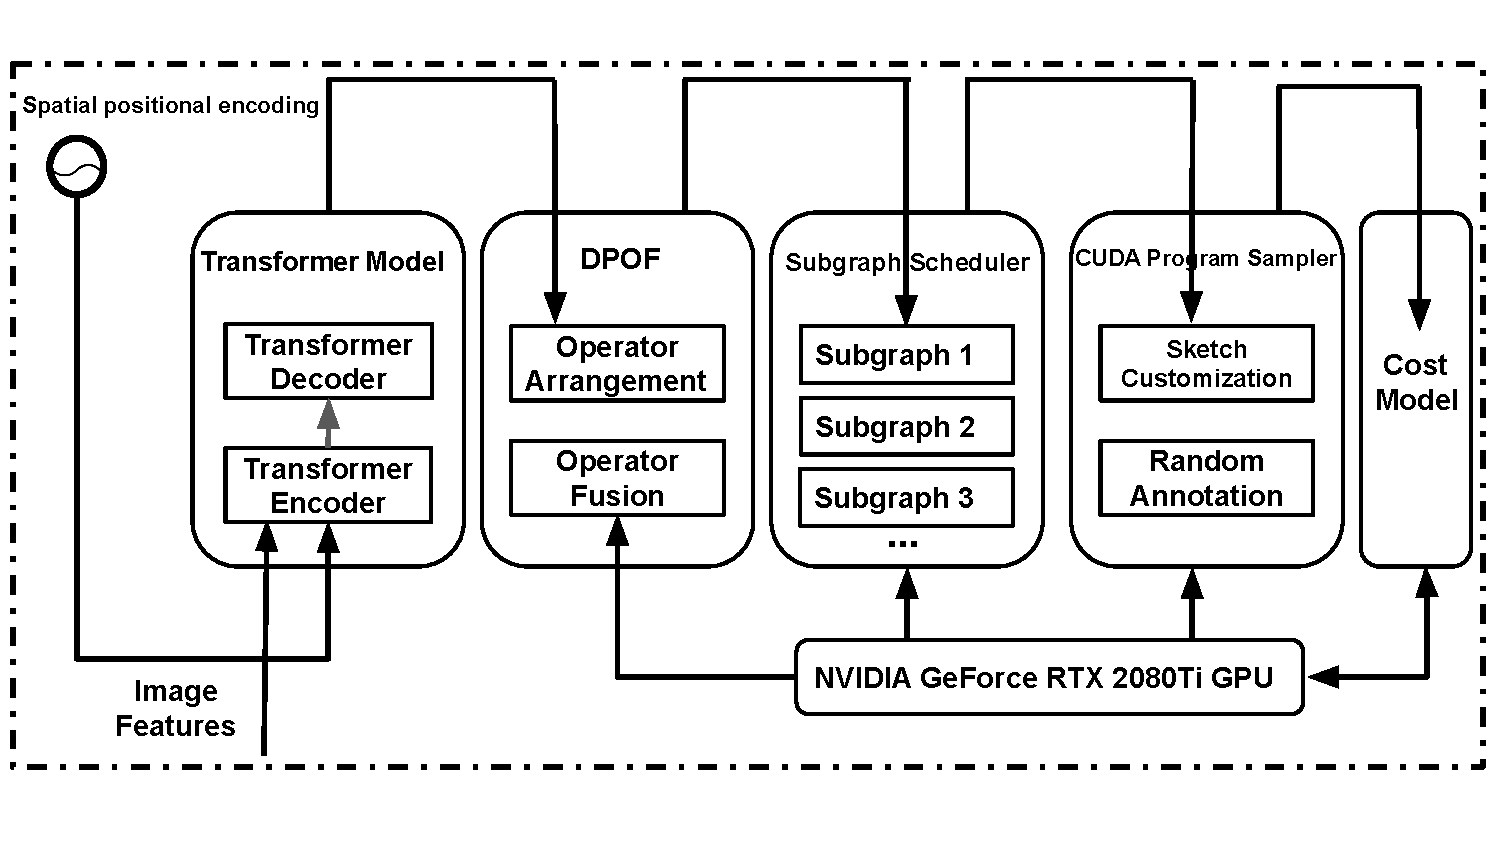
\includegraphics[height=7cm, width=18cm]{figs/fig3}
    \caption{xxx}
    \label{fig:fig3}
\end{figure*}


\subsection{DPOF}


\subsubsection{Operator Arrangement}
% computation graph -> computation queue and move all of the placeholder operators -> set all of the operators in queue as opaque type and get the 
% maximum phases of our scheduling.
To find an optimized schedule for a transformer model, we first use topological sort algorithm to obtain the execution order of the computation operators in the 
original graph. Second, we build a computation queue to store these operators. It is convenient for us to find a good scheduling based on the queue rather than 
computation graph.For the placeholder variables, we do not consider them because they only stores the input and output of the computation results and does 
not mitigate the performance of the whole graph. As mentioned in the operator pattern section, each operator has its own type and the different types of the same 
operator make the difference in the runtime. Third, we set all of the operators as opaque type and assume that there is no fusion relationship with each other.
The size of such queue is the maximum number phase of the scheduling algorithm which is defined in problem definition.


\subsubsection{Operator Fusion}
When we get the execution order of the computation operators and the maximum number phase of our schedule, we partition the original computation graph
$G=(V, E)$ into $V-V^{'}$ and $V^{'}$. The edges in set of $V-V^{'}$ have the pointing relationship with the edges in set of $V{'}$. That is, all of the 
edges start from $V-V^{'}$ and end up with $V{'}$. We call $V{'}$ the segmentation set.

\begin{figure}[htbp]
    \centering
    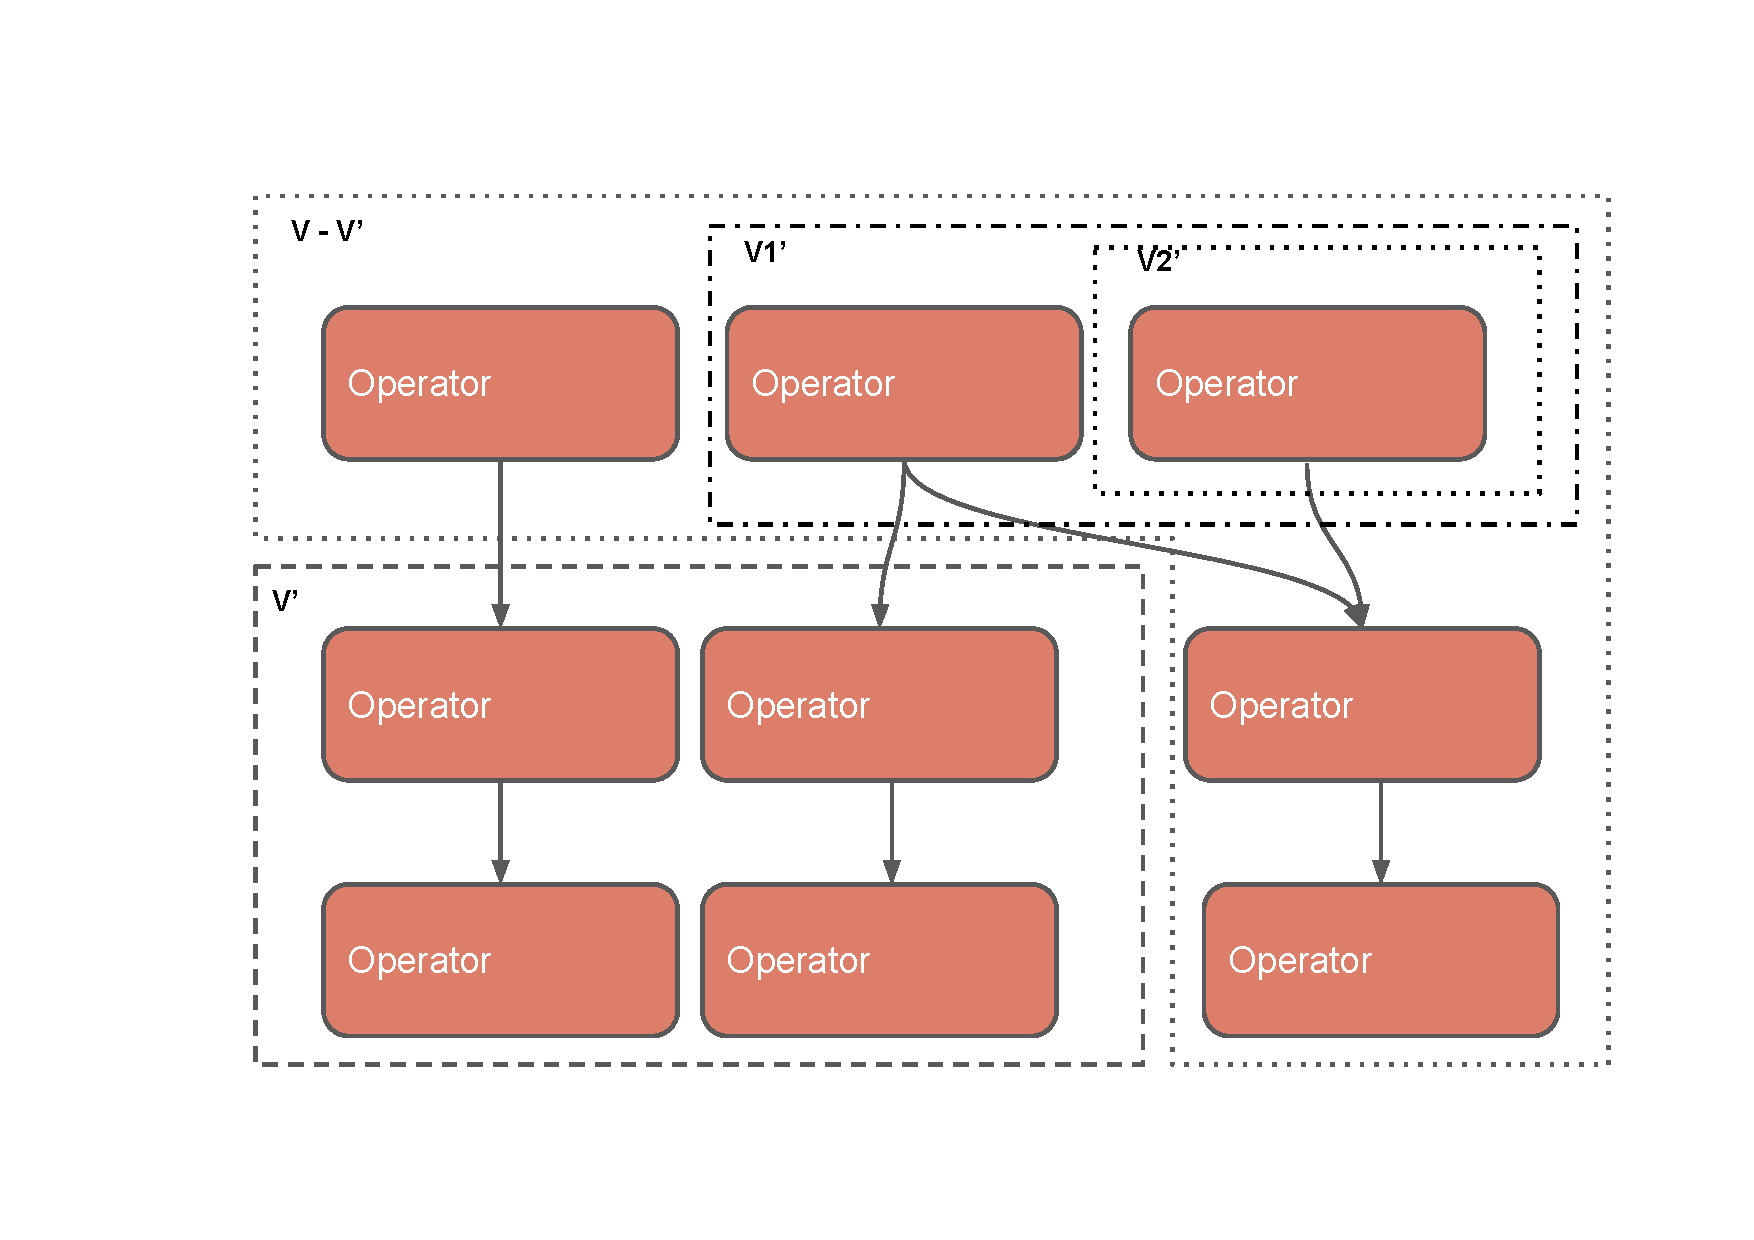
\includegraphics[height=6cm, width=6cm]{figs/fig2}
    \caption{xxx}
    \label{fig:fig1}
\end{figure}

The relationship is illustrated in Figure xxx. We can find that there are lots of segmentaion sets in the computation graph. Following the dynamic programming
pipeline, we can enumerate the segmentaion sets $V{'}$ of $V$ and convert the problem to a sub-problem that attains the optimial schedule for $V-V^{'}$. Therefore,
the whole graph can be sovled by employing the segmentaion set recursively. \\
We define $dp[V]$ as the latency of the graph with the node set $V$ under an optimial schedule $S$. And then we define $temp[V^{'}]$ as the latency of 
phase $(V^{'}, F)$. In the representation, $F$ is the better fusion strategy for the segmentaion set $V^{'}$. Consequently, we can get the state transition 
equation as follows,
\begin{equation}
    dp[V] = min_{ v \in V^{'}}(dp[V-V^{'}] + \sum_{v}temp[v]),    
\end{equation}
where $v$ is the node in segmentaion set $V^{'}$ and the boundary value of the state transition equation is $dp[\varnothing] = 0$. In order to get the optimial
schedule, we store the each node $v$ in segmentaion set $V^{'}$ that can make the latency of each $V$ in $action[V]$.
Following the above information, we implement the operator fusion scheduling as shown in Algorithm xxx.

% \begin{algorithm}[htb]
%     \caption{Operator Fusion Strategy}
%     \label{fra:Framwork}
%     \begin{algorithmic}[1]
%       \Require
%         % The set of positive samples for current batch, $P_n$;
%         % The set of unlabelled samples for current batch, $U_n$;
%         % Ensemble of classifiers on former batches, $E_{n-1}$;
%         a computation graph $G=(V, E)$ with the opaque type for ${\forall v \in V}, pattern(v) = 0$;
%       \Ensure
%         % Ensemble of classifiers on the current batch, $E_n$;
%         A operator fusion strategy with the type of each operator $v \in V, pattern(v)$;

%     \State \textbf{function} func1(G)
%       \State Extracting the set of reliable negative and/or positive samples $T_n$ from $U_n$ with help of $P_n$;
%       \label{code:fram:extract}
%       \State Training ensemble of classifiers $E$ on $T_n \cup P_n$, with help of data in former batches;
%       \label{code:fram:trainbase}
%       \State $E_n=E_{n-1}cup E$;
%       \label{code:fram:add}
%       \State Classifying samples in $U_n-T_n$ by $E_n$;
%       \label{code:fram:classify}
%       \State Deleting some weak classifiers in $E_n$ so as to keep the capacity of $E_n$;
%       \label{code:fram:select} \\
%       \Return $E_n$;
%     \end{algorithmic}
% \end{algorithm}


\begin{algorithm}[htb]
    \setstretch{0.8}
    \caption{Operator Fusion Strategy}
    \begin{algorithmic}[1]
        \Require
        % The set of positive samples for current batch, $P_n$;
        % The set of unlabelled samples for current batch, $U_n$;
        % Ensemble of classifiers on former batches, $E_{n-1}$;
        a computation graph $G=(V, E)$ with the opaque type for ${\forall v \in V}, pattern(v) = 0$;
      \Ensure
        % Ensemble of classifiers on the current batch, $E_n$;
        A operator fusion strategy with the type of each operator $v \in V, pattern(v)$;
        \\
        \State Defining $dp[\varnothing] \gets 0$, $dp[V] \gets +\infty$, $action[V] \gets \varnothing$;
        \State Defining $S \gets \left[\varnothing\right]$ (a stack to store the phase of optimial schedule for operator fusion);
    \\
    \Function {SelectSchedule}{$G$}
        \State $V$ = all operators in computation graph $G$;
        \State Scheduler(V);
        % \State $S = \left[ \qquad \right]$
        \While{$V \neq \varnothing $}
            \State $V^{'}, F = action[V]$;
            \State Put phase $(V^{'}, F)$ into the stack $S$;
            \State $V = V - V^{'}$
        \EndWhile
        \State \Return {the Fusion Strategy $S$}

    \EndFunction
    \\
    \Function{Scheduler}{V}
        \If{$dp[V] \neq +\infty$} 
            \State \Return{dp[V]}
        \EndIf
        \ForAll{$v \in V^{'}$}
            \State $T_{V^{'}}, F_{V^{'}} = PhasePartition(V^{'})$
            \State $T_{V} = Scheduler(V-V^{'}) + \sum_{v_i \in V^{'}}T_{V^{'}}$
            \If{$T_{V} \le dp[V]$}
                \State $dp[V] = T_{V}$
                \State $action[V] = (V^{'}, F_{V^{'}})$
            \EndIf
        \EndFor;
        \State \Return{$dp[V]$}
    \EndFunction
    \\
    \Function{PhasePartition}{$V^{'}$}
        % \If{ $type(v_i \in V^{'} ) == compute\_matmul$}
        %     \State Partition $V^{'}$ into separate groups based cut point $v_i$;
        % \Else
        %     \State xxx
        % \EndIf

        \ForAll{$operators \ v_i \in \ V^{'}$} 
            \If{$pattern(v_i, v_j)\neq opaque$} 
                \State $T_{fused(i, j)} = Runtime(pair(v_i, v_j))$
            \Else
                \State $T_{fused(i, j)} = +\infty$
            \EndIf
        \EndFor
        % \State \Return{$T_{fused(i, j)}, "fused v_i and v_j into an operator"$}        
        \State \Return{$T_{fused(i, j)}, pattern(v_i, v_j)$}        

    \EndFunction




    %     \If {$left < right$}
    %         \State $middle \gets (left + right) / 2$
    %         \State $result \gets result +$ \Call{MergerSort}{$Array, left, middle$}
    %         \State $result \gets result +$ \Call{MergerSort}{$Array, middle, right$}
    %         \State $result \gets result +$ \Call{Merger}{$Array,left,middle,right$}
    %     \EndIf
    %     \State \Return{$result$}
    % % \EndFunction

    %   \ForAll {$c$ such that $c\in RecentMBatch(E_{n-1})$}
    %     \label{code:TrainBase:getc}
    %     \State $T=T\cup PosSample(c)$;
    %     \label{code:TrainBase:pos}
    %   \EndFor;
    %   \For{$i=1$; $i<n$; $i++$ }
    %     \State $//$ Your source here;
    %   \EndFor
    %   \For{$i=1$ to $n$}
    %     \State $//$ Your source here;
    %   \EndFor
    %   \State $//$ Reusing recent base classifiers.
    %   \label{code:recentStart}
    %   \While {$(|E_n| \leq L_1 )and( D \neq \phi)$}
    %     \State Selecting the most recent classifier $c_i$ from $D$;
    %     \State $D=D-c_i$;
    %     \State $E_n=E_n+c_i$;
    %   \EndWhile
      \label{code:recentEnd}
    \end{algorithmic}
  \end{algorithm}


\subsection{Subgraph Scheduler}

% Using topological sort to build a queue, then extract feature from each operator to generate schedule. 
% When tunning a transformer model, our goal is to reduce the model's latency, meeting latency requirements, or
% minimizing tuning time when tuning no longer improves the performance of subgraph significantly.

{\color{red} Change the cost model of the task scheduler, make it early stopping for large kernel}
A transformer model can be partitioned into kinds of independent subgraphs (such as batch\_matmul + softmax). In the process of 
optimization, spending time to tune some subgraphs does not improve the whole performance of entire computation graph. As mentioned in the Ansor paper, there
are two reasons: (1) the subgraph is not a performance bottleneck, or (2) tuning brings only minimal improvement in the subgraph\'s performance. Therefore, we
should dynamically allocate different amounts of time resources to different kinds of subgraphs. A subgraph can appear multiple times in models because of the 
characteristics of the transformer. We define a task as a process performed to generate high-performance programs for a subgraph. It means that obtaining a high
optimized transformer needs completing lots of tasks. 

When tuning a set of subgraphs in transformer, we combine three types of goals together: (1) reducing the latency of transformer, (2) meeting latency requirements
for a set of subgraphs, or (3) minimizing tuning time when tuning no longer improves the performance of transformer significantly. We define $t$ as the allocation
vector, where $t_i$ is the number of time units spent on \textit{i-}th task and the initial value of $t$ is $(1, 1, ..., 1)$. We also define $g_{i}(t)$ as the minimum subgraph latency under the \textit{i-}th task
with $t_i$ time units. Therefore, the latency of the subgraphs $f(g_{1}(t), g_{2}(t), ..., g_{n}(t))$ can describe the end-to-end latency of a transformer model and our
goal is to minimize this function. In order to minimize the end-to-end latency of the transformer, we define the following objective function:
\begin{equation}
    % dp[V] = min_{ v \in V^{'}}(dp[V-V^{'}] + \sum_{v}temp[v]),   
    % f = \sum\limits_{j=1}^{m} max \left[\sum\limits_{i \in S(j)}w_{i} \times max(g_{i}(t), ES(g_{i}, t)), L_{j} \right] 
    f =  max \left[\sum\limits_{i = 1}^{n} w_{i} \times max(g_{i}(t), ES(g_{i}, t)), L_{j} \right] 
    %{\sum_{i \in S(j) w_{i} \times max(g_{i}(t), ES(g_{i}, t))}}
\end{equation}
In the above function, $w_i$ is the number of appearances of task $i$ in the transformer. We define $L_{j}$ as the latency requirement of subgraph $j$, meaning that we do not want to spend tuning time on a subgraph if its latency 
has already met the requirement. In order to achieve the effect of early stopping, we also define a function named ${ES(g_i, t)}$ by looking at the history of latecny
of \textit{i-}th task. Unlike the objective functions defined in Ansor, we first make a comparison between meeting the requirement and early stopping, and then optimize
each task sequentially. Finally, we use a scheduling algorithm based on gradient descent to efficiently optimize the objective function mentioned in Ansor.


\subsection{Program Sampler}

{\color{red} Add the new derivation rules to generate new sketchs:
cross-thread reduction to optimize batch matmul and softmax}

To sample tensor program effectively that can cover a large search space, we also define a hierarchical search
space with two levels like Anosr: \textbf{sketch} and \textbf{annotation}. We define the high-level structures 
of tensor programs as our sketches and set millions of low-level choices (\textit{e.g.}, blocking size, virtual thread tiling, cooperative fetching) as our annotations. The generated tensor program is composed of two top. The component of the first level are sketches generated
by the derivation rules which are designed on GPU platform. The detail information of the second level are randomly annotated from the annotation
space. In order to generate sketches for a subgraph of transformer (DAG), we visit all the computation nodes in a topological order and iteratively build 
a generation structure. For compute-intensive or the nodes with a high chance of data reuse (such as batch matrix multiplication, convolution2d), we build 
a classic tile and fusion structures for them as the sketch. It is worth noting that some new nodes for caching will also be introduced to increase memory 
usage during the generation of sketch.



Figure \ref{fig:fig4} shows an example of the generated sketches for a common subgraph which contains matrix multiplication and softmax operations. For the example subgraph, 
the sorted order of the five nodes in the DAG is \textbf{(A, B, M, S, D)}. To get the sketches for the subgraph, we start from output node \textbf{D} and apply the rules
defined in Ansor to the computation node one by one. We can get the generated sketch 1 by Anosr in the Figure xxx. From the generated sketch 1, we find that the matrix 
multiplication and softmax operations are performed separately, and they are not integrated into a computation kernel. Fortunately, the derivation-based sketch generation 
in Ansor is flexible enough to generate the required structures for emerging algorithms and hardware, because Ansor allows users to register new derivation rules and integrate
them seamlessly with existing rules. In the next section, I will describe in detail about our sketch customization and fused policy.
% We will explain the sampling process of \textbf{scaled dot-product attention} for GPUs 
\begin{figure*}[htbp]
    \centering
    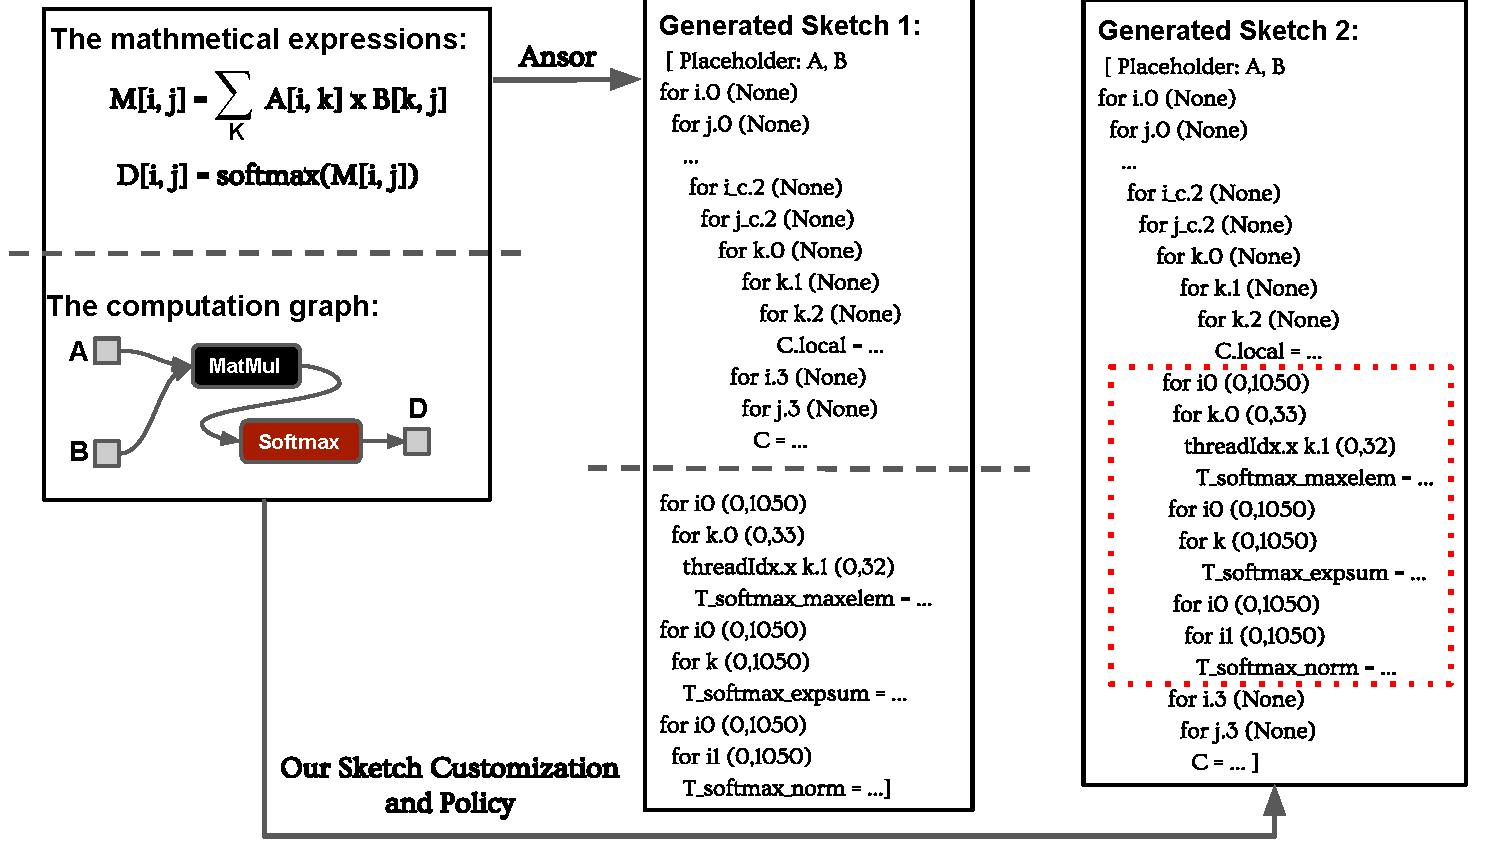
\includegraphics[height=6cm, width=10cm]{figs/fig4}
    % 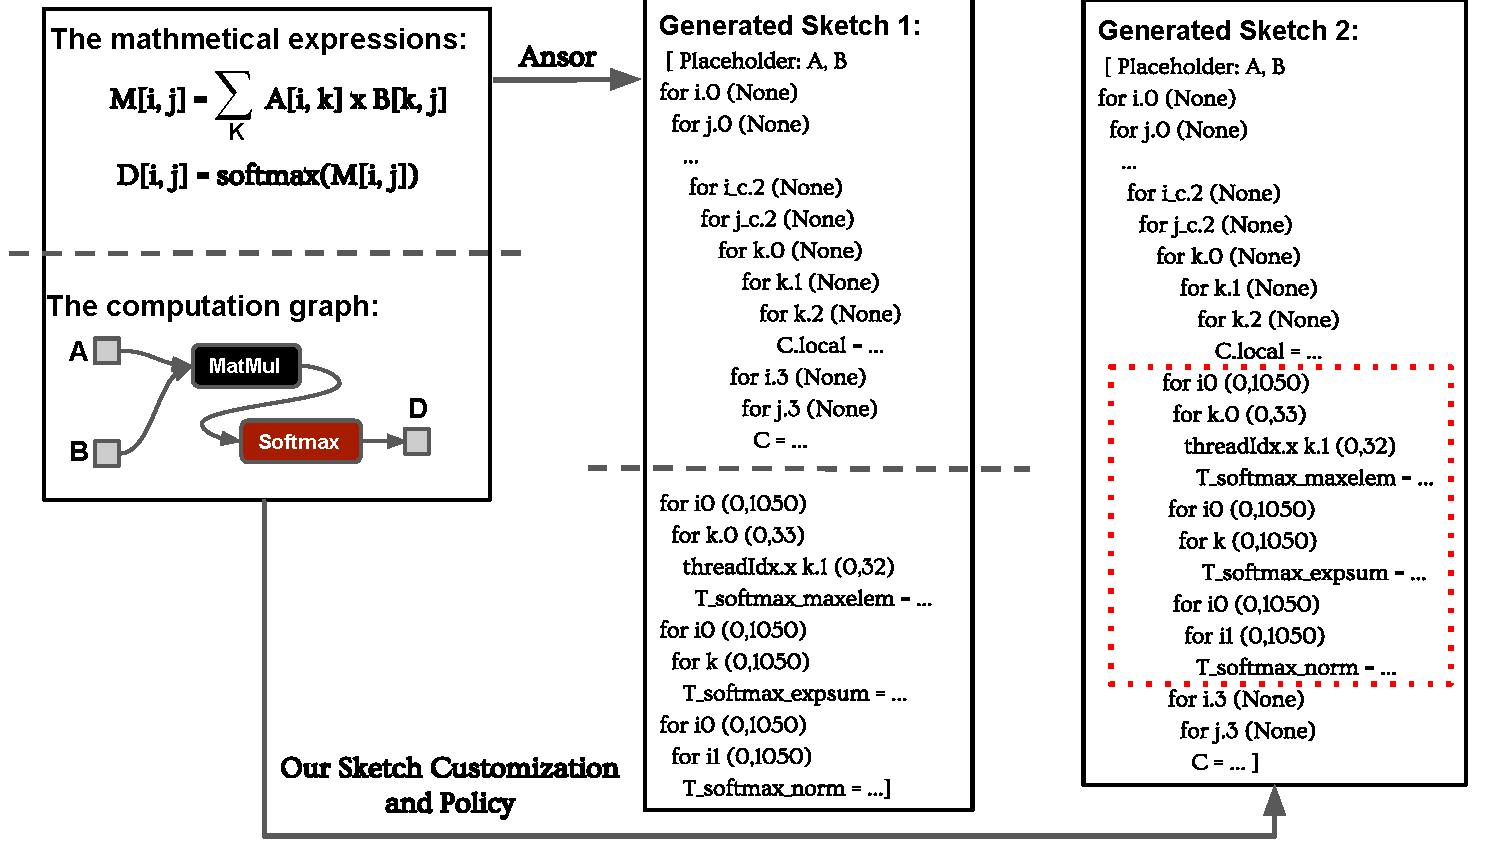
\includegraphics[width=10cm]{figs/fig4}
    % \hspace{1in}
    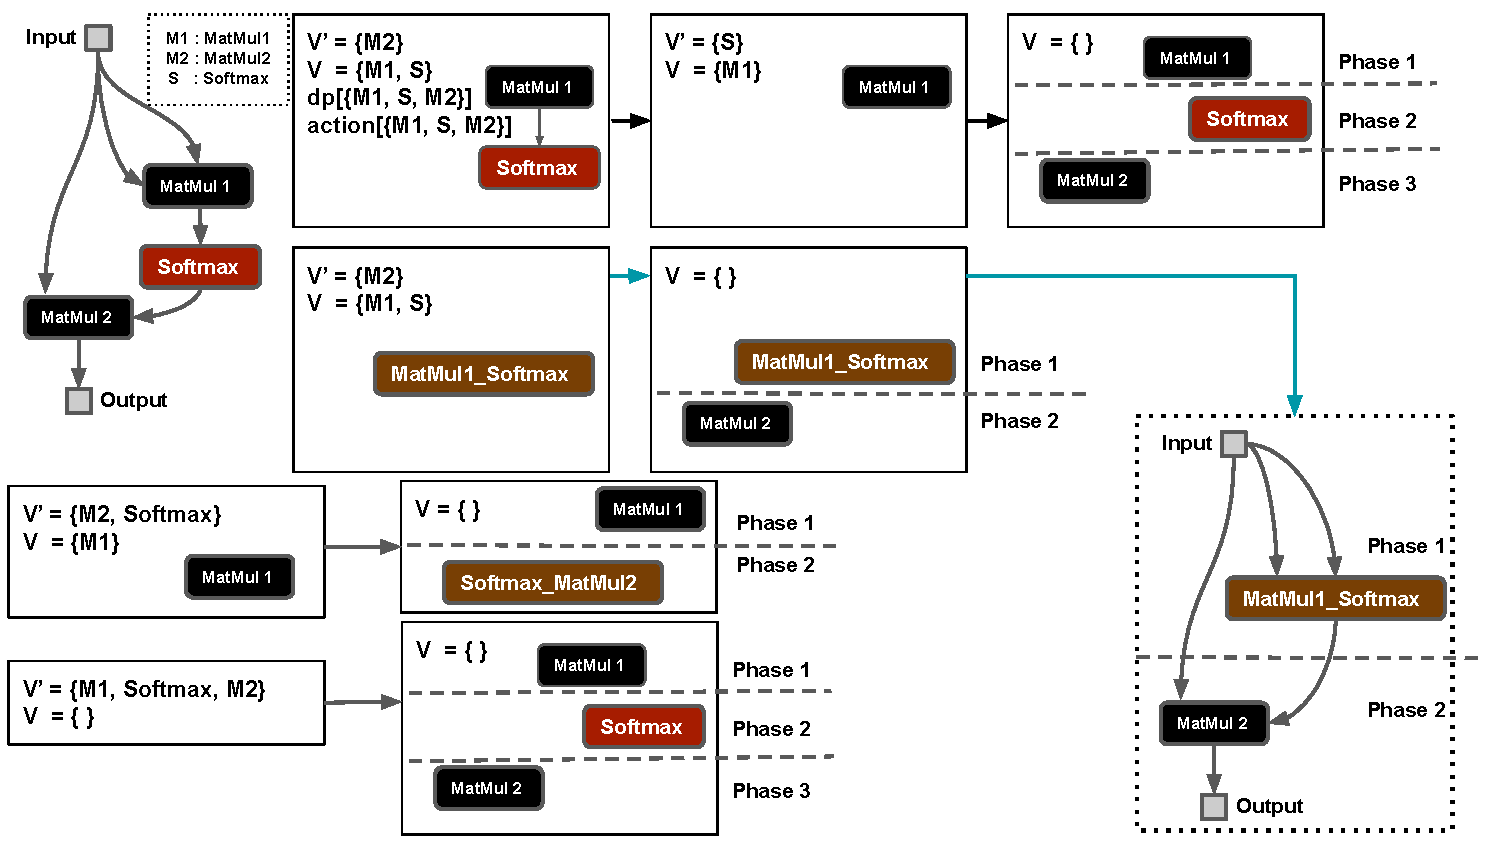
\includegraphics[height=6cm, width=8cm]{figs/fig7}
    \caption{xxx}
    \label{fig:fig4}
\end{figure*}

% \begin{figure}[htbp]
% \centering
% \begin{minipage}[t]{0.48\textwidth}
% \centering
% \includegraphics[width=6cm]{test1.jpg}
% \caption{World Map}
% \end{minipage}
% \begin{minipage}[t]{0.48\textwidth}
% \centering
% \includegraphics[width=6cm]{test2.jpg}
% \caption{Concrete and Constructions}
% \end{minipage}
% \end{figure}



\subsubsection{Sketch Customization} 

The default sketch configuration of Anosr for the multi-level tiling structure to match the GPU backend is SSSRRSRS.
The first three S corresponds to BlockIdx, virtual thread, and ThreadIdx in GPUs programming model, respectively.
The SSSRRSRS tile structure for matrix multiplication expands the original %3-level loop \textbf{(i, j, k)} into a 19-level loop \textbf{(i_{0},j_{0},i_{1},j_{1}, ...)}.
Even if we do not enumerate the loop order, this multi-level tiling structure can take this into consideration. In the example subgraph shown in Figure xxx, we design an effective
operator fusion policy for the sketch generation. The SSSR-RSRS tile structure is for batch matrix multiplication and softmax operators. In order to fuse more opertors and make 
full use of GPUs computation resources, we insert a caching node with the SS-S tile structure to store the sketch generation of the matrix multiplication in it and then 
send it to the sketch generation of softmax to get the final sketch of the subgraph. From the Figure xxx, we can find that the generation sketch of matrix multiplication 
and softmax operators are fused into the same computation kernel.




% \subsubsection{Random Annotation} 
The sketches generated by our customization are incomplete programs because they only have thread parallel structures without specific 
value of these parameters. Therefore, we should turn them into complete programs and then fine-tuning and evaluate the complete programs. 
We randomly pick one sketch from the a list of generated sketches by our customizations. As for the outer loops, we use parallelize intrinstics to optimize them. And for the inner loops, we use vectorize and unroll intrinstics to optimize them.
All valid parameters for the random values are sampled from a uniform distribution.



\subsection{Performance Tuner}

{\color{red} Evolutionary Search and Learned Cost model (same as Ansor)}


\textbf{ML-Based Cost Model and Evolutionary Search:} 
One way to find the best scheduling of the tensor program from a large search space is by auto-tuning. Therefore, a cost model is particularly 
important in the process of evaluating the performance of programs. The extracted features include arithmetic features and memory access features, which
includes number of float operations, number of integer operations, vectorization related features, unrolling related features, parallelization related features,
GPU thread binding related features, buffer access feature, allocation related feature. More specifically, we use weighted squared error as the loss function and 
the loss function of the model $f$ on a sampled program $P$ with throughput $y$ can be defined as follow:
\begin{equation}
    loss(f, P, y) = w_{p}(\sum\limits_{s \in S(P)} f(s) - y)^{2},
\end{equation}
where $S(P)$ is the set of innermost non-loop statements in $P$ and we train a gradient boosting decision tree as the underlying model $f$. In the actual
calculation, we directly make $y$ approximately equal to $w$.\\

A search policy is necessary for the performance tuner. The evolutionary search leverages mutation
and crossover mechanism to generate a new set of candidates repeatedly for several rounds and outputs a small set of programs with the highest scores. The generated
programs will be compiled and measured on the GPU backend to obtain the real running time cost. In the meantime, the collected from the training is then used to
improve the performance of cost model. Therefore, we adopt the search policy which is introduced in Ansor by designing correponding evolution operations to rewrite
and fine-tune the sampled programs.


\label{sec:algo}



\section{Evaluation Results}
\subsection{Experimental Setup}

We evaluate the fusion optimization and kernel generation mechanisms on three modern image recognition tasks with transformers: DETR, SETR, and ViT. %Table xxx and Table xxx summarize workload characteristics.
We use cuDNN V7.6.5, CUDA 11.0, NVIDIA driver 460.67, and adopt TensorRT V7.0.0.11 and TVM 0.8, as well as the TensorRT version as 
baselines for our performance comparison study. All evaluation results are collected on a NVIDIA GeForce RTX 2080Ti GPU. 

% We compare Automatic-E2EF against the state-of-art search frameworks and hardware-specific manual libraries. In the meantime, we evaluate the search
% efficiency of each module designed in Automatic-E2EF. 



% \subsection{Graph Fusion Analysis}

% \subsection{Kernel tunning Analysis}

\subsection{Subgraph Benchmark}
{\color{red} multi-head attention, encoder and decoder}

We perform the subgraph benchmark on two three subgraphs in tranformer. The multi-head attenion (mha) is a subgraph consisting of \textbf{h} attention heads in parallel
to attend to different learned projections of a sequence. The \textit{encoder} is a subgraph consisting of \textbf{n} identical layers. Each layer has two sub-layers. The first is a mha mechanism, and the second is a simple,
positionwise fully connected feed-forward network. The \textit{decoder} is a subgraph consisting of \textbf{n} identical layers. It inserts a third sub-layer, which performs multi-head attention over the output of 
the encoder layer. We select three different shape configurations which corresponds to the image recognition benchmarks and two batch sizes, run auto-tuning with up to xxx
measurement trails per test case, and report the normalized performance. In the meantime, we use the same set of paramters on the baseline framework. \\
Figure xxx shows that our dynamic programming operator fusion technqiue outperforms manual libraries (tensorrt) and other search frameworks (ansor )by xxx.


\subsection{End-to-End Performance}
\textbf{Workloads.} we benchmark the end-to-end inference execution time of three image recognition models with transformers, which include DETR ResNet-50
for object detection, SETR ResNet-50 for semantic segmentation, and ViT for image classification. We report the results for batch size 1. Table xxx shows the 
number of encoders, the number of decoders, and the input shape of the tensor for each network. \\



{\color{red} DETR:}

Attention mechanisms in the transformer models are the key components which model relations between feature representations of different location of objects.
%For the study 
we choose ResNet-50-based DETR model with \textbf{6} encoder, \textbf{6} decoder layers and width \textbf{256}. 
To be comparable in the number of paramters we choose a model with 6 encoder and 6 decoder layers of width 256 with 8 attention heads. \\

{\color{red} SETR:}
asada \\

{\color{red} ViT:}
ASDASD \\



\textbf{Baselines.} asdada \\
\textbf{Results.} asdasd \\
\textbf{Abliation study.} asdasd \\



\label{sec:result}

% ==================== table1 =====================
% architecture of the model
% \newpage
% \begin{table*}[htbp]
%     \caption{architecture of the model}
%     \centering
%     \scalebox{0.75}{
%     \begin{tabular}{l|l|l|l|l|l|l|l|l|l|l}
%     \hline
%     model               & encoder & decoder & width & nhead & input shape           & patch & transformer input                                                                     & mha input                                                                                                            & encoder input          & decoder input                                                                             \\ 
%     \hline
%     \hline
%     resnet50-based DETR & 6       & 6       & 256   & 8     & {[}1, 3, 800, 1333{]} & N/A   & \begin{tabular}[c]{@{}l@{}}src {[}1050,1, 256{]} \\ tgt {[}100,1, 256{]}\end{tabular} & \begin{tabular}[c]{@{}l@{}}query {[}1050, 1, 256{]}\\ key {[}1050, 1, 256{]}\\ value {[}1050, 1, 256{]}\end{tabular} & src {[}1050, 1, 256{]} & \begin{tabular}[c]{@{}l@{}}tgt {[}100, 1, 256{]}\\ memory {[}1050, 1, 256{]}\end{tabular} \\
%     \hline
%     SETR-Naive          & 24      & 1       & 1024  & 16    & {[}1, 3. 768, 768{]}  & 16    & \begin{tabular}[c]{@{}l@{}}src {[}2304,1, 1024{]} \\ tgt {[}2304, 1, 1024{]}\end{tabular} & \begin{tabular}[c]{@{}l@{}}query {[}2304, 1, 1024{]}\\ key {[}2304, 1, 1024{]} \\ value {[}2304, 1, 1024{]}\end{tabular} &   src {[}2304, 1, 1024{]}    &   {[}2304, 1, 1024{]}                                 \\
%     \hline
%     ViT-Base-16         & 12      & 0       & 768   & 12    & {[}1, 3, 224, 224{]}  & 16    & \begin{tabular}[c]{@{}l@{}}src {[}197, 1, 768{]} \\ tgt {[}197, 1, 768{]}\end{tabular}    & \begin{tabular}[c]{@{}l@{}}query {[}197, 1, 768{]}\\ key {[}197, 1, 768{]} \\ value {[}197, 1, 768{]}\end{tabular}  &     src {[}197, 1, 768{]}   &     N/A                                                    \\ 
%     \hline
%     \end{tabular}
%     }
% \end{table*} 

\newpage
\begin{table*}[htbp]
    \caption{architecture of the model}
    \centering
    \resizebox{1.02\textwidth}{!}{
        \renewcommand{\arraystretch}{1.0}{
        \begin{tabular}{l|l|l|l|l|l|l|l|l|l|l}
        \toprule
        model & encoder & decoder & width & nhead & input shape & patch & transformer input   & mha input & encoder input & decoder input \\ 
        \midrule
        resnet50-based DETR & 6 & 6 & 256 & 8 & {[}1, 3, 800, 1333{]} & N/A & \begin{tabular}[c]{@{}l@{}}src {[}1050,1, 256{]} \\ tgt {[}100,1, 256{]}\end{tabular} & \begin{tabular}[c]{@{}l@{}}query {[}1050, 1, 256{]}\\ key {[}1050, 1, 256{]}\\ value {[}1050, 1, 256{]}\end{tabular} & src {[}1050, 1, 256{]} & \begin{tabular}[c]{@{}l@{}}tgt {[}100, 1, 256{]}\\ memory {[}1050, 1, 256{]}\end{tabular} \\
        \midrule
        SETR-Naive          & 24      & 1       & 1024  & 16    & {[}1, 3. 768, 768{]}  & 16    & \begin{tabular}[c]{@{}l@{}}src {[}2304,1, 1024{]} \\ tgt {[}2304, 1, 1024{]}\end{tabular} & \begin{tabular}[c]{@{}l@{}}query {[}2304, 1, 1024{]}\\ key {[}2304, 1, 1024{]} \\ value {[}2304, 1, 1024{]}\end{tabular} &   src {[}2304, 1, 1024{]}    &   {[}2304, 1, 1024{]}                                 \\
        \midrule
        ViT-Base-16         & 12      & 0       & 768   & 12    & {[}1, 3, 224, 224{]}  & 16    & \begin{tabular}[c]{@{}l@{}}src {[}197, 1, 768{]} \\ tgt {[}197, 1, 768{]}\end{tabular}    & \begin{tabular}[c]{@{}l@{}}query {[}197, 1, 768{]}\\ key {[}197, 1, 768{]} \\ value {[}197, 1, 768{]}\end{tabular}  &     src {[}197, 1, 768{]}   &     N/A                                                    \\ 
        \bottomrule
        \end{tabular}
    }}
\end{table*}

\begin{table*}[htbp]
    \caption{batch matrix multiplication and softmax in MHA}
    \centering
    \begin{tabular}{|l|l|l|l|l|l|l|l|}
    \hline
    layers (encoder) & GFLOPS & \#params & mAP  & PyTorch JIT & TensorRT & Ansor & Our method  \\ \hline
    3                & 81     & 37.4M    & 40.1 & 5.64        & 2.87     & 2.71  & 2.37        \\ \hline
    6                & 86     & 41.3M    & 40.6 & 11.45       & 5.65    & 6.13  & 5.25         \\ \hline
    12               & 95     & 49.2M    & 41.6 & 23.17       & 11.37    &  12.35     &  9.98            \\ \hline
    \end{tabular}
\end{table*}


\begin{table*}[htbp]
    \caption{dynamic programming for operator fusion on DETR}
    \centering
    \scalebox{0.75}{
    \begin{tabular}{|l|l|l|l|l|l|l|l|}
    \hline
             & encoder & weights & decoder & weights & transformer & weights  & measurement trails \\ \hline
    Ansor    &     9                &   [6, 6, 6, 6, 6, 12, 12, 6, 6]  &       13   & [18, 6, 6, 6, 6, 18, 18, 6, 6, 6, 6, 6, 6]  &           22               &      [18, 6, 6, 6, 6, 19, 19, 6, 6, 6, 6, 6, 6, 6, 6, 6, 13, 13, 6, 6, 6, 6]                  &        10000            \\ \hline
    AutoGTCO &              &                        &                      &                     &                          &                        &       8790             \\ \hline
    \end{tabular}
    }
\end{table*}


\begin{table*}[htbp]
    \caption{DETR Acceleration}
    \centering
    \begin{tabular}{|l|l|l|l|l|l|}
    \hline
                & MHA  & Encoder & Decoder & Transformer & Speedup \\ \hline
    PyTorch JIT & 0.53 & 12.96   & 15.75   & 23.67       & -   \\ \hline
    TensorRT    & 2.05 & 5.65    & 5.65    & 7.73        & 1.00    \\ \hline
    Ansor       & 1.07 & 6.13    & 1.58    & 6.78        & 1.12x   \\ \hline
    AutoGTCO    & 0.83 & 5.25    & 1.35    & 5.60        & 1.27x   \\ \hline
    \end{tabular}
\end{table*}


\begin{table}[htbp]
    \caption{image recognition with transformers acceleration}
    \centering
    \scalebox{0.85}{
    \begin{tabular}{|l|l|l|l|l|}
    \hline
                   & PyTorch JIT & TensorRT & Ansor & AutoGTCO \\ \hline
    DETR-ResNet-50 & 23.67       &  7.73    & 6.78  & 5.60     \\ \hline
    SETR-Naive     &             &          &       &          \\ \hline
    ViT-Base-16x16 &             &          &       &          \\ \hline
    \end{tabular}
    }
\end{table}

\newpage
\section{Related Work}

\textbf{Graph-level optimization.} 
Graph-level optimizations, inspired from classical loop optimizations, is known to improve performance in other domains. They treat each operator in the computational
graph as a basic unit and implement optimization to at each subgraph without changing the intramural representation of original operators. In the high-performance computing domain, [30] formulated GPU kernel fusion as an combinatorial search problem, and search the candidate for an optimized fusion-kernel. In image processing and computer vision 
domains, [22, 23] formulated the image processing pipeline as a standard graph-cut problem. In machine learning domain, [7] introduced a kernel fusion mechanism to
generate efficient kernel code for a specific computation pattern. In the compiler domain, XLA compiler can handle more general computation pattern, but offers
only basic capability for fusion and kernel generation. However, XLA relies on empirical rules to analyze fusion possibilities, and does not support kernel generation 
with the specific operator pattern, such as elementwise, gemm, and reduction. TVM compiler can also implement operator fusion optimization. It uses Relay[] to make 
all of the rule-based graph-level optimization in compiler pass with lots of engineering workload. In the meantime, it relies on disjoint-set and
post-dominator tree in a very complex way, which may ignore lots of opportunities to improve the end-to-end performance. As for graph-level optimization, the common optimizations include layout transformation, elementwise operator fusion, constant folding, and automatic 
generation of graph substitution. The graph-level optimizations are orthogonal to the tensor-level optimizations and can be combined to boost the performance
of whole system. MetaFlow performs functional-preserving graph transformations to optimize neural network architectures. In order to reduce accesses to GPU memories,
it merges operators with the same input variable and make them implement more parallelly. TASO further designs an automated generation of substitution rules and 
it explores more mathematically equivalent neural network structures of the input one comparing to MetaFlow. MetaFlow and TASO treat the whole computation 
graph as a whole part and search for highly optimized substitution subgraphs for the original part. However, we do not want to change the structure of the original
neural network and find some new subgraphs to replace them, which seems like a neural network search on hardware. We leave the joint optimization of graph substitution 
and tensor-level optimization as future work.

\textbf{Tensor-level optimization.}
Halide proposes a scheduling language that can describe loop optimization primitives. Manual optimization and automatic search algorithm can be feasible in
this domain specific language. Currently, halide has three different versions of auto-scheduler based on various search techniques. TVM utilizes a similar scheduling
language, which is named as tensor expression, and it also requires users to design all kinds of template for different hardware backends. Optimized tensor programs
are generated by template-guided saerch framework AutoTVM. Ansor also explores kernel fusion
with tuning approach under limited patterns supported. FlexTensor introduces some general templates that can address a set of specific operators. It is obvious that
these templates can solve single operator efficiently rather than the subgraphs involving multiple operators.
People can provide schedules and Halide, TVM, Ansor, FlexTensor can tune the parameters automatically. However, 
the optimization of operator fusion is not the schedule for a single operator itself, but how to group different types of operator into fusion patterns and store 
them together into a single kernel on specific hardware backend efficiently.



\label{sec:result}


\section{Conclusions}
Existing deep learning compilers do optimization on computation graph-level by greedy methods designed by human experts, which are strictly execution performance 
increasing. This apporch misses potential performance gains from more effective operators fusion strategies.
This work tackles the problem from two aspects. First, we introduce a novel dynamic programming algorithm to explore and optimize fusion strategies. 
Together with operator fusion optimizations, we propose new sketch generation rules and a search policy for the batch matrix multiplication and softmax operators in 
transformer subgraphs, which are capable of fusing them into large computation units, then mapping and transforming them into 
efficient CUDA kernels. In order to get a high-performance and end-to-end compilation flow, a learned cost model is used to fine-tune the performance of each kernel 
in the code generation stage. Experiments results on three real-world image recognization tasks with transformers are encouraging. Overall, AutoGTCO can reach up to
1.27x execution performance speedups compared to the current state-of-the-art deep learning library TensorRT.
  

\label{sec:conclu}





%\balance
{
\bibliographystyle{IEEEtran}
\bibliography{./ref/Top-sim,./ref/addition}
}


\end{document}



